\documentclass[conference]{IEEEtran}
\IEEEoverridecommandlockouts
\usepackage{cite}
\usepackage{amsmath,amssymb,amsfonts}
\usepackage{graphicx}
\usepackage{textcomp}
\usepackage{xcolor}
\usepackage{booktabs}
\usepackage{url}
\usepackage{tikz}
\usetikzlibrary{positioning,arrows.meta,fit}

\begin{document}

\title{Multi-Crop Leaf Localization with YOLOv8 and Zero-Shot Vision-Language Crop Identification for Plant Disease Diagnosis}

\author{
\IEEEauthorblockN{Ashmit Janjirkar}
\IEEEauthorblockA{\textit{Dept. of Information Technology}\\
\textit{Dwarkadas J. Sanghvi College of Engineering}\\
Mumbai, India\\
ashmit.janjirkar@gmail.com}
\and
\IEEEauthorblockN{Hitansh Gada}
\IEEEauthorblockA{\textit{Dept. of Information Technology}\\
\textit{Dwarkadas J. Sanghvi College of Engineering}\\
Mumbai, India\\
\textit{[email]}}
\and
\IEEEauthorblockN{Aryan Gada}
\IEEEauthorblockA{\textit{Dept. of Information Technology}\\
\textit{Dwarkadas J. Sanghvi College of Engineering}\\
Mumbai, India\\
\textit{[email]}}
\and
\IEEEauthorblockN{Urav Jain}
\IEEEauthorblockA{\textit{Dept. of Information Technology}\\
\textit{Dwarkadas J. Sanghvi College of Engineering}\\
Mumbai, India\\
\textit{[email]}}
}

\maketitle

\begin{abstract}
Automated leaf-disease diagnosis usually assumes that the crop is already known and that the leaf was photographed against a clean background. Neither holds for a farmer's photo of a field. We work on the step before diagnosis: finding the leaves in an image and deciding which of five crops grown widely in Maharashtra (sugarcane, wheat, maize, rice and soybean) they belong to. Five CC~BY~4.0 Roboflow Universe datasets are merged into one crop-level detection set of 11,346 images and 40,561 boxes, and 3,020 polygon annotations that the training framework would reject are converted to boxes. A hash audit of the sources' own splits found that 20.3\% of validation and 25.0\% of test images have an exact, near-duplicate or flipped/rotated copy in an earlier split. We regroup the duplicates so that none crosses a split, and release the new split with a per-image hash manifest. On the original split, YOLOv8n (3.0~M parameters, 8.2~GFLOPs) reached 0.754 mAP@50 and 0.522 mAP@50-95 on validation after 50 epochs; given the leakage, these numbers are optimistic. A vision-language model (Llama~4 Scout), restricted to the five crop names, identifies the crop zero-shot, and a threshold rule chooses between it and the detector: when the detector's confidence falls below $\tau$, the VLM's answer is used. EigenCAM maps give a first look at what the detector attends to. The practical lesson is that merged public plant datasets should be deduplicated before their scores are believed.
\end{abstract}

\begin{IEEEkeywords}
plant disease detection, object detection, YOLOv8, vision-language models, zero-shot classification, dataset deduplication, explainable AI
\end{IEEEkeywords}

%=====================================================================
\section{Introduction}

Agriculture contributes roughly 11--12\% of Maharashtra's gross state domestic product and employs close to half of its workforce. Sugarcane, wheat, maize, rice and soybean are among the state's most widely grown crops, and all of them get leaf diseases such as rusts, blights, leaf spots and viral mosaics. Catching these early limits their spread, but that usually takes an expert looking at the plant, and most smallholder farmers cannot get one quickly.

Deep learning recognizes plant diseases well under controlled conditions \cite{mohanty2016, sujatha2025}, but two problems show up in practice. Most systems cover a single crop \cite{phadikar2008, sethupathy2016, khanal2024}, so the user has to know what they photographed and pick the matching model. And models trained on laboratory images with plain backgrounds lose much of their accuracy on field photos full of leaves, soil, shadow and clutter \cite{mohanty2016, singh2020plantdoc}. Localizing the leaves first helps with the second problem, since a later classifier can then look at cropped regions instead of the whole frame.

This paper handles that first step for five crops at once: find the leaf regions, then say which crop they come from. The contributions are:
\begin{enumerate}
\item A reproducible merge of independently annotated public datasets into one five-class YOLO dataset. It records provenance and licences, converts polygons to boxes, and runs a hash-based leakage audit (MD5, perceptual hash under flips and rotations, Roboflow source groups) that produces a split with no cross-split duplicates.
\item A YOLOv8n detector (3.0~M parameters) for crop-level leaf localization, reported with per-epoch training curves and per-crop validation AP.
\item Zero-shot crop identification with a vision-language model (VLM) whose output is limited to the five crops, plus a confidence-threshold rule that settles disagreements between the VLM and the detector.
\end{enumerate}

Section~\ref{sec:related} covers related work and Section~\ref{sec:method} the dataset, detector, VLM and fusion rule. Section~\ref{sec:results} gives results, Section~\ref{sec:discussion} discusses limitations and Section~\ref{sec:conclusion} concludes.

%=====================================================================
\section{Related Work}\label{sec:related}

\textit{Classical approaches.} Phadikar and Sil \cite{phadikar2008} identified rice diseases by segmenting infected regions and classifying them with a self-organizing map, reaching about 82\% accuracy. Sethupathy and Veni \cite{sethupathy2016} detected mango leaf diseases with OpenCV, using K-means segmentation and an SVM classifier. Both rely on hand-crafted features and cover one crop.

\textit{Deep learning classification.} Mohanty \textit{et al.} \cite{mohanty2016} trained CNNs on the PlantVillage dataset \cite{hughes2015plantvillage} (over 50,000 images, 14 crops, 26 diseases) and got very high accuracy on held-out laboratory images, but accuracy fell sharply on images taken under other conditions. Sujatha \textit{et al.} \cite{sujatha2025} compared machine learning and deep learning models for leaf disease detection, and the deep models came out ahead consistently. Nagababu \textit{et al.} \cite{nagababu2024} and Bonkra \textit{et al.} \cite{bonkra2023} also describe CNN pipelines for disease diagnosis.

\textit{Detection on field images and domain shift.} PlantDoc \cite{singh2020plantdoc} offers 2,598 field images with bounding boxes for 13 plant species and 27 classes, and showed how much harder detection on real-world images is than laboratory classification. Khanal \textit{et al.} \cite{khanal2024} trained YOLOv8 models on more than 20,000 paddy images and report an average detection mAP@50 of 69\%. The Global Wheat Head Detection dataset \cite{david2020gwhd} pooled images from many institutions and countries because detectors trained at one site transfer poorly to others. The same caution applies to our multi-source setting: scores on splits drawn from the same sources say little about independent field photos.

\textit{Open-vocabulary detection.} CLIP \cite{radford2021clip} learns a joint image--text space by contrastive pre-training and can classify images zero-shot from class names. OWL-ViT \cite{minderer2022owlvit}, Grounding DINO \cite{liu2024groundingdino} and YOLO-World \cite{cheng2024yoloworld} carry the idea over to detection and find objects described in free text; YOLO-World does so in real time. In principle such a detector could replace both of our modules. We use image-level classification with a general VLM instead. It needs no labelled data, its constrained answer can be compared directly with the detector's crop label, and in our data crop identity is an image-level property anyway, since each image shows a single crop. Testing an open-vocabulary detector on the same split is left for future work.

\textit{Merging heterogeneous datasets.} Zhou \textit{et al.} \cite{zhou2022unidet} train one detector on several datasets and learn a unified label space from their partly overlapping taxonomies. Label-Aligned Transfer (LAT) \cite{kennerley2026lat} projects source annotations into a target label space, using dataset-specific detectors as privileged proposal generators together with a semantic feature fusion module. Our case is simpler, because each source covers exactly one crop and the class mapping is unambiguous. What merge-and-relabel cannot fix is \emph{annotation style}: one source boxes whole leaves, another boxes lesions. LAT-style label transfer could help there (Section~\ref{sec:discussion}).

%=====================================================================
\section{Methodology}\label{sec:method}

Fig.~\ref{fig:pipeline} shows the pipeline. The per-crop datasets are merged, audited for duplicates and re-split; YOLOv8n is trained on the result and exported to ONNX. At inference the detector sees every image, and the VLM is called only when the detector is not confident.

\begin{figure}[t]
\centering
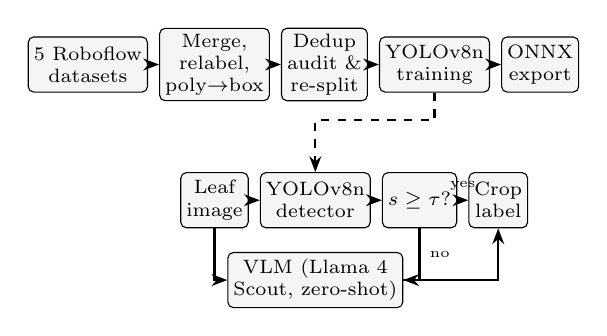
\begin{tikzpicture}[
  node distance=4mm and 1.4mm,
  box/.style={draw, rounded corners=2pt, align=center, font=\scriptsize, minimum height=7mm, inner sep=2pt, fill=gray!8},
  arr/.style={-{Stealth[length=2mm]}, thick}]
\node[box] (src) {5 Roboflow\\datasets};
\node[box, right=of src] (merge) {Merge,\\relabel,\\poly$\to$box};
\node[box, right=of merge] (dedup) {Dedup\\audit \&\\re-split};
\node[box, right=of dedup] (train) {YOLOv8n\\training};
\node[box, right=of train] (onnx) {ONNX\\export};
\draw[arr] (src) -- (merge);
\draw[arr] (merge) -- (dedup);
\draw[arr] (dedup) -- (train);
\draw[arr] (train) -- (onnx);
\node[box, below=9mm of merge] (img) {Leaf\\image};
\node[box, right=of img] (det) {YOLOv8n\\detector};
\node[box, right=of det] (gate) {$s\ge\tau$?};
\node[box, right=of gate] (out) {Crop\\label};
\node[box, below=3mm of det] (vlm) {VLM (Llama 4\\Scout, zero-shot)};
\draw[arr] (img) -- (det);
\draw[arr] (det) -- (gate);
\draw[arr] (gate) -- node[above, font=\tiny]{yes} (out);
\draw[arr] (img.south) |- (vlm.west);
\draw[arr] (gate.south) |- node[pos=0.25, right, font=\tiny]{no} (vlm.east);
\draw[arr] (vlm.east) -| (out.south);
\draw[arr, dashed] (train.south) -- ++(0,-3.5mm) -| (det.north);
\end{tikzpicture}
\caption{Pipeline. Top: dataset construction and training. Bottom: inference; the VLM decides when the detector's top confidence $s$ is below $\tau$.}
\label{fig:pipeline}
\end{figure}

\subsection{Dataset Construction and Provenance}

No public detection dataset covers all five crops, so we take one YOLO-format dataset per crop from Roboflow Universe (Table~\ref{tab:sources}), all under CC~BY~4.0. The maize source has 10,000 images; to keep it in proportion with the other crops we draw a fixed random subset of 1,200 (seed 42) that keeps its train/validation/test ratios. Each source labels healthy and diseased leaf regions with its own disease classes, and the class indices overlap, so the files cannot simply be concatenated. The sources also draw their boxes very differently (Fig.~\ref{fig:samples}).

\begin{figure*}[t]
\centering
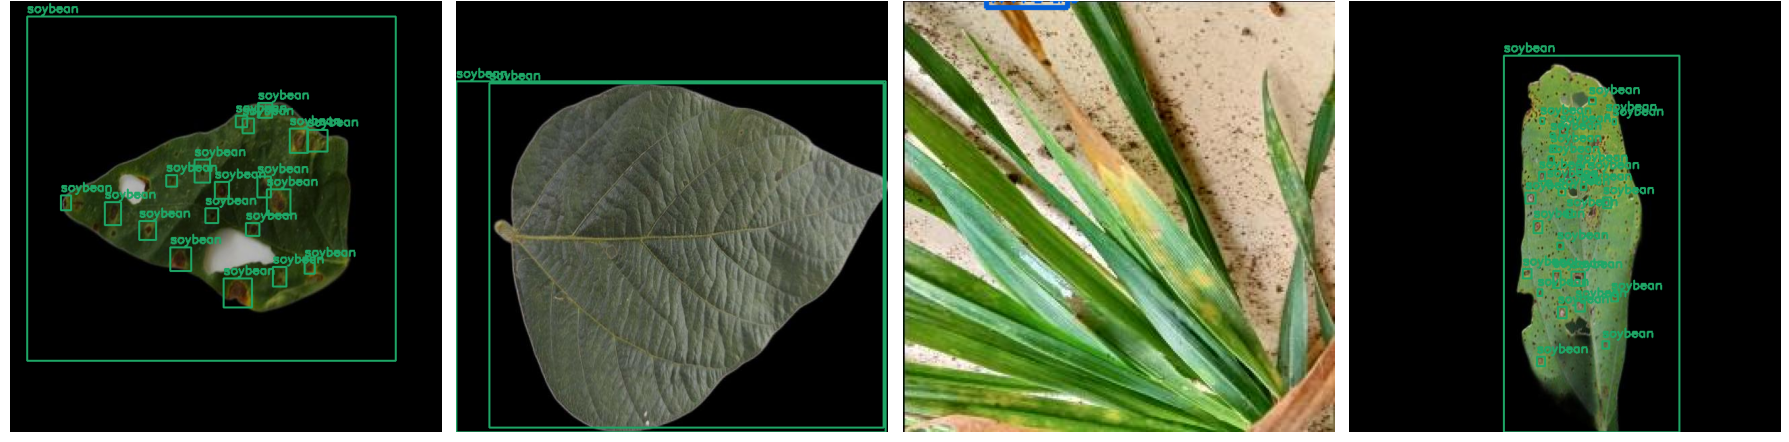
\includegraphics[width=0.95\textwidth]{fig_samples.png}
\caption{Ground-truth annotations from the merged dataset, all relabelled to the crop class. Boxes range from whole leaves to individual lesions, sometimes on the same image (first and fourth panels).}
\label{fig:samples}
\end{figure*}

\begin{table}[t]
\caption{Source Datasets (Roboflow Universe, all CC BY 4.0)}
\label{tab:sources}
\centering
\footnotesize
\setlength{\tabcolsep}{2.5pt}
\begin{tabular}{llrrr}
\toprule
Crop & Roboflow project (ver.) & Images & Boxes & Area$^*$ \\
\midrule
Sugarcane & sugar-cane-disease-model (v2) \cite{ds_sugarcane} & 3,011 & 3,529 & 52.7\% \\
Wheat & wheat-plant-diseases (v6) \cite{ds_wheat} & 1,774 & 2,168 & 27.7\% \\
Maize & maize-leaf-diseases (v1) \cite{ds_maize} & 1,200 & 1,200 & 98.3\% \\
Rice & rice-plant-disease-det.\ (v1) \cite{ds_rice} & 1,440 & 1,667 & 47.2\% \\
Soybean & soy-leaf-disease (v15) \cite{ds_soybean} & 3,921 & 31,997 & 0.1\% \\
\midrule
Total & & 11,346 & 40,561 & \\
\bottomrule
\end{tabular}
\\[1mm]{\footnotesize $^*$Median box area as a share of the image, on the training split.}
\end{table}

The merge script (\texttt{merge\_datasets.py}) does four things:
\begin{enumerate}
\item \textit{Layout detection.} It handles split-first exports (\texttt{train/images}, \texttt{valid/images}), images-first layouts (\texttt{images/train}) and unsplit folders.
\item \textit{Relabelling.} Every object from the source for crop $c$ gets class index $c \in \{0,\dots,4\}$ (sugarcane, wheat, maize, rice, soybean).
\item \textit{Polygon-to-box conversion.} Some exports put segmentation polygons and box rows in the same label file. The training framework rejects such files as corrupt, and in our first training run it dropped 53 of them. The script now replaces each polygon (3,020 rows in 2,709 files) with its axis-aligned bounding box, clipped to the image, so no annotation is lost.
\item \textit{Name isolation.} Each file name is prefixed with its crop. This prevents collisions, and the ground-truth crop of any image can be read from its name.
\end{enumerate}
The resulting labels encode \emph{crop identity} for each annotated leaf region. Disease identity is dropped; Section~\ref{sec:discussion} discusses that choice.

\subsection{Leakage Audit and Group-Aware Split}

Roboflow exports often include several augmented copies of one photograph (named \texttt{<orig>\_jpg.rf.<hash>}), and field datasets often include burst shots of the same scene. To check whether such copies cross split boundaries, we hash every image with MD5, which catches exact copies, and with a 64-bit perceptual hash (pHash). Two images count as near-duplicates if their pHashes differ in at most 4 bits. Validation and test images are also compared under all eight flips and $90^\circ$ rotations, because the sources used those as augmentations. Last, files are grouped by their Roboflow source stem.

In the splits shipped with the sources, 223 of 1,098 validation images (20.3\%) and 138 of 551 test images (25.0\%) have a duplicate in an earlier split, and 40 Roboflow source groups span more than one split. Most matches are wheat and rice images: flipped or rotated copies, or burst shots taken seconds apart. We inspected 12 random pairs at the loosest threshold (distance 4). Nine were clear duplicates; the other three were single leaves photographed against the same white background, so the audit leans toward over-flagging. No duplicate pair links two different crops.

We join duplicate pairs into groups with union--find. A group that spans several splits moves entirely into one of them: training if it contains a training image, validation otherwise. Table~\ref{tab:split} shows the result, and re-running the audit on the new split finds no cross-split duplicates. The price is small rice and wheat test sets (29 and 33 images), so per-crop numbers for those two crops will be noisy. The merge, audit and split scripts are released with a manifest of per-image MD5 and pHash values.

\begin{table}[t]
\caption{Original and Group-Aware Clean Splits (Images)}
\label{tab:split}
\centering
\setlength{\tabcolsep}{4pt}
\begin{tabular}{lrrrrrr}
\toprule
& \multicolumn{3}{c}{Original} & \multicolumn{3}{c}{Clean} \\
\cmidrule(lr){2-4}\cmidrule(lr){5-7}
Crop & Train & Val & Test & Train & Val & Test \\
\midrule
Sugarcane & 2,640 & 247 & 124 & 2,741 & 182 & 88 \\
Wheat & 1,492 & 186 & 96 & 1,638 & 103 & 33 \\
Maize & 840 & 240 & 120 & 840 & 240 & 120 \\
Rice & 1,260 & 120 & 60 & 1,347 & 64 & 29 \\
Soybean & 3,465 & 305 & 151 & 3,487 & 291 & 143 \\
\midrule
Total & 9,697 & 1,098 & 551 & 10,053 & 880 & 413 \\
\bottomrule
\end{tabular}
\end{table}

\subsection{Detector}

We use YOLOv8 \cite{yolov8}, a single-stage, anchor-free detector, in its smallest (\textit{nano}) size: 130 layers, 3.01~M parameters and 8.2~GFLOPs at $640\times640$ input, starting from COCO-pretrained weights. Nano suits the intended setting of low-cost hardware and edge devices.

The loss is the YOLOv8 default, a weighted sum of a CIoU box-regression term, a binary cross-entropy classification term and a distribution focal loss (DFL) term:
\begin{equation}
\mathcal{L} = \lambda_{\text{box}}\mathcal{L}_{\text{CIoU}} + \lambda_{\text{cls}}\mathcal{L}_{\text{BCE}} + \lambda_{\text{dfl}}\mathcal{L}_{\text{DFL}},
\end{equation}
with $\lambda_{\text{box}}=7.5$, $\lambda_{\text{cls}}=0.5$ and $\lambda_{\text{dfl}}=1.5$.

To imitate the variety of farmers' field photos we use mosaic composition (probability 1.0, switched off for the last 10 epochs of the schedule), MixUp (0.1), copy-paste (0.1), HSV jitter (hue 0.015, saturation 0.7, value 0.4), rotation ($\pm10^\circ$), translation (0.1), scaling (0.5), shear ($2^\circ$), and horizontal and vertical flips (0.5 each). The framework adds light blur, grayscale and CLAHE at probability 0.01.

\subsection{Training Setup}

Training ran on one NVIDIA Tesla T4 (15 GB) in Google Colab with Ultralytics 8.4.118, PyTorch 2.11 and automatic mixed precision, at $640\times640$ with batch size 16. The framework chose the optimizer itself: an SGD variant with initial learning rate 0.01, momentum 0.9 and weight decay $5\times10^{-4}$, after a 3-epoch warm-up. The schedule was 100 epochs, but the limits of the free GPU session stopped the first run, on the original split, after epoch 50 (about 3.2 minutes per epoch). Training now saves a checkpoint to persistent storage every five epochs, so a session reset no longer ends a run.

\subsection{Zero-Shot Crop Identification with a VLM}

The detector needs labelled data for every crop it knows; the VLM needs none. We use Llama 4 Scout \cite{llama4}, a mixture-of-experts multimodal model with 17B active parameters, through the Groq inference API \cite{groq}. The image is sent base64-encoded with a system prompt that:
\begin{itemize}
\item limits the answer to the five crops, with an explicit \textit{unknown} for images that show none of them;
\item asks for strict JSON with the fields \textit{crop}, \textit{confidence} (an integer from 0 to 100) and \textit{reason}. An answer outside the five classes, or one that does not parse, becomes \textit{unknown}.
\end{itemize}
Decoding uses temperature 0.1 and at most 100 output tokens, which keeps answers short and stable. The VLM gives one label per image with no boxes, and it needs a network connection, whereas the detector runs offline.

\subsection{Fusion Rule}

Let $s$ be the highest confidence among the detector's boxes on an image and $\hat{y}_{\text{det}}$ that box's class, and let $\hat{y}_{\text{VLM}}$ be the VLM's answer. The image-level crop label is
\begin{equation}
\hat{y} = \begin{cases} \hat{y}_{\text{det}} & \text{if } s \ge \tau,\\ \hat{y}_{\text{VLM}} & \text{otherwise (including no boxes).} \end{cases}
\end{equation}
The detector gets priority because it runs offline and localizes the leaves. The VLM is asked only when the detector is unsure, which cuts network calls and cost. We pick $\tau$ from $\{0.25, 0.4, 0.5, 0.6, 0.75\}$ by image-level accuracy on the validation split, which leaves the test split for the final measurement.

\subsection{Evaluation Protocol}

A prediction is a true positive if its intersection-over-union (IoU) with a ground-truth box of the same class reaches the threshold; precision is $P = TP/(TP+FP)$ and recall $R = TP/(TP+FN)$. Average precision (AP) is the area under the precision--recall curve. We report its mean over classes at IoU 0.5 (mAP@50) and averaged over IoU thresholds from 0.50 to 0.95 in steps of 0.05 (mAP@50-95), with the framework's default confidence threshold of 0.001 and NMS IoU of 0.7. Image-level crop accuracy takes the filename prefix as ground truth. The released evaluation script (\texttt{experiments/run\_all.py}) also covers test-set and per-crop evaluation, VLM accuracy and its agreement with the detector, the fusion rule and ONNX Runtime CPU latency, and it logs the output file behind every reported value.

%=====================================================================
\section{Results}\label{sec:results}

\subsection{First Training Run (Original Split)}

Table~\ref{tab:results} gives validation metrics of the first run at selected epochs, and Fig.~\ref{fig:curves} the full curves. The best epoch, 49, reaches mAP@50 0.754, mAP@50-95 0.522, precision 0.769 and recall 0.747 on 1,127 validation images with 3,802 objects. This run used an earlier copy of the merged data with 51 more images (11,397), kept the sources' leaky original split, and lost the 53 mixed polygon files. Because of the leak the numbers are optimistic, and they cannot be compared with results on the clean split.

\begin{table}[t]
\caption{Validation Metrics of the First Run (Original Split)}
\label{tab:results}
\centering
\begin{tabular}{rcccc}
\toprule
Epoch & Precision & Recall & mAP@50 & mAP@50-95 \\
\midrule
1 & 0.302 & 0.516 & 0.414 & 0.223 \\
10 & 0.664 & 0.630 & 0.625 & 0.399 \\
20 & 0.749 & 0.695 & 0.698 & 0.448 \\
30 & 0.772 & 0.716 & 0.725 & 0.477 \\
40 & 0.767 & 0.734 & 0.733 & 0.499 \\
\textbf{49} & \textbf{0.769} & \textbf{0.747} & \textbf{0.754} & \textbf{0.522} \\
50 & 0.768 & 0.755 & 0.748 & 0.516 \\
\bottomrule
\end{tabular}
\end{table}

\begin{figure}[t]
\centering
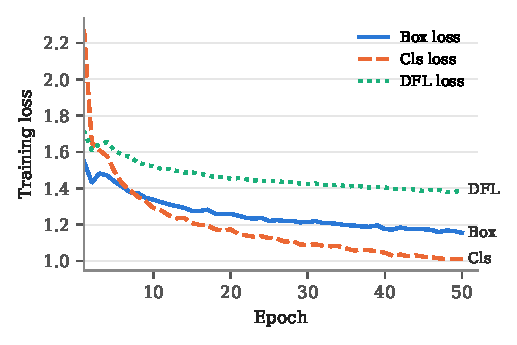
\includegraphics[width=\columnwidth]{fig_loss.pdf}\\[-1mm]
{\footnotesize (a) Training losses}\\[2mm]
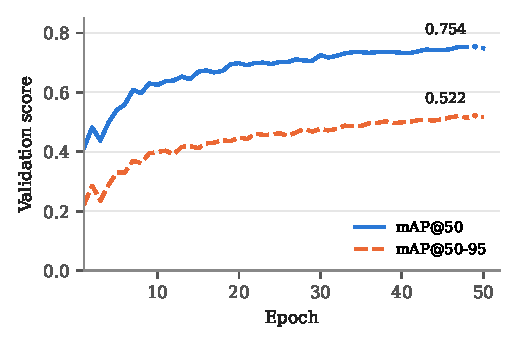
\includegraphics[width=\columnwidth]{fig_map.pdf}\\[-1mm]
{\footnotesize (b) Validation mAP; dots mark the best epoch (49)}
\caption{Training dynamics of the first YOLOv8n run over 50 epochs.}
\label{fig:curves}
\end{figure}

Most of the gain comes early. mAP@50 climbs from 0.414 to 0.625 in the first 10 epochs and to 0.698 by epoch 20, then adds only about 0.03 over the last 20. At epoch 50 all three training losses were still falling (box 1.155, classification 1.012, DFL 1.388) and the validation metrics had not levelled off. That tells us the run stopped before convergence. It does not tell us the remaining 50 epochs would have helped, since validation scores can also flatten or drop once mosaic is switched off near the end.

\subsection{Per-Crop Validation AP (Second, 30-Epoch Run)}

\begin{figure}[t]
\centering
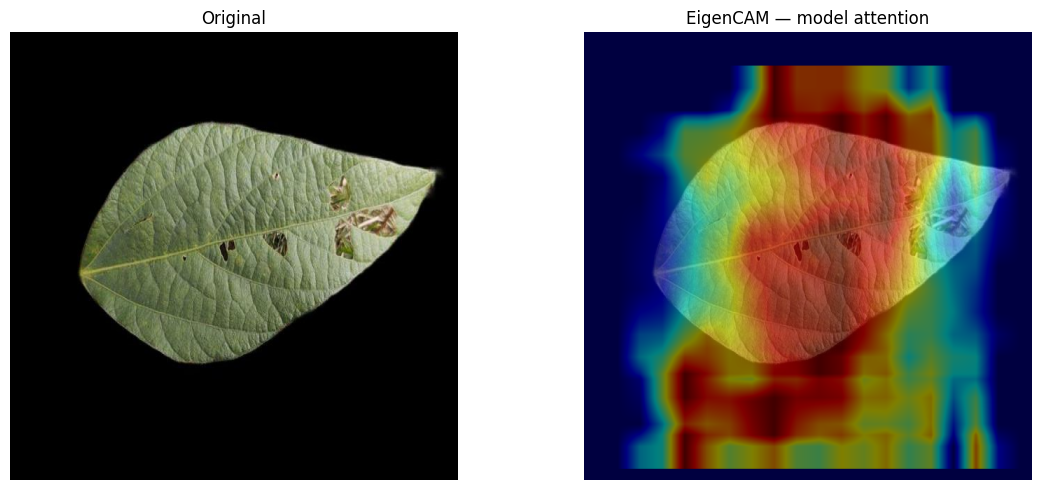
\includegraphics[width=\columnwidth]{fig_eigencam.png}
\caption{EigenCAM attention of YOLOv8n on a soybean test image (left: input; right: map overlaid).}
\label{fig:eigencam}
\end{figure}

A second YOLOv8n run used the same data, split and augmentation, but batch size 32 and a 30-epoch schedule, which it completed. Table~\ref{tab:percrop} gives its per-crop results on the same validation set. Overall it reaches mAP@50 0.746 and mAP@50-95 0.511, close to the first run, and the same leakage caveat applies.

\begin{table}[t]
\caption{Per-Crop Validation Metrics of the 30-Epoch Run (Original Split)}
\label{tab:percrop}
\centering
\setlength{\tabcolsep}{4pt}
\begin{tabular}{lrrcccc}
\toprule
Crop & Images & Boxes & P & R & mAP@50 & mAP@50-95 \\
\midrule
Sugarcane & 247 & 298 & 0.849 & 0.826 & 0.871 & 0.575 \\
Wheat & 183 & 225 & 0.678 & 0.468 & 0.554 & 0.281 \\
Maize & 240 & 240 & 0.987 & 1.000 & 0.995 & 0.874 \\
Rice & 117 & 128 & 0.680 & 0.664 & 0.637 & 0.504 \\
Soybean & 305 & 2,911 & 0.725 & 0.653 & 0.671 & 0.320 \\
\midrule
All & 1,127 & 3,802 & 0.784 & 0.722 & 0.746 & 0.511 \\
\bottomrule
\end{tabular}
\end{table}

The differences between crops track annotation style more than crop difficulty. Maize boxes cover almost the whole image (Table~\ref{tab:sources}), and maize is detected almost perfectly (mAP@50 0.995), which says little about localization. Soybean, labelled at lesion level, has the lowest mAP@50-95 (0.320), because small boxes are hard to match tightly. Wheat has the lowest mAP@50 (0.554) and recall (0.468), even though it is the crop most affected by leakage.

Fig.~\ref{fig:samples} shows the underlying difference: some sources box whole leaves, others box many small lesions on one leaf. Table~\ref{tab:sources} puts numbers on it. The median maize box covers 98\% of the image, with one box per image, while the median soybean box covers 0.1\%, with 8.0 boxes per image and 74.5\% of soybean training boxes under 1\% of the image area. This mix of scales is a likely reason mAP@50-95, which rewards tight boxes, stays well below mAP@50.

\subsection{Explainability}

To see which image regions drive the detector we use EigenCAM \cite{muhammad2020eigencam}, which projects a layer's activations onto their first principal component. It needs no gradients and no class score, which suits a detector whose output is a set of boxes. We apply it to the last C2f block before the detection head of the 30-epoch checkpoint (Table~\ref{tab:percrop}). Fig.~\ref{fig:eigencam} shows the result for a soybean test leaf. The strongest attention sits on the central blade and the insect-damaged patch, but a clear band also lands on the plain black background below the leaf. One map cannot tell us whether the detector relies on leaf features or on context such as background or box scale (Section~\ref{sec:discussion}). Measuring, for each crop, how much of the map falls inside ground-truth boxes is future work.

\subsection{Efficiency}

The model has 3.01~M parameters and 8.2~GFLOPs. Exported to ONNX, it runs on CPU or edge hardware through ONNX Runtime without the training framework.

%=====================================================================
\section{Discussion and Limitations}\label{sec:discussion}

\textit{Crop-level labels.} The biggest limitation is that the detector predicts the crop, not the disease. Collapsing the sources' disease labels into crop classes is what made it possible to merge datasets with incompatible label schemes, and the result still finds leaf and lesion regions across all five crops. Telling diseases apart needs a second stage, for example a per-crop classifier run on the detected regions and selected by the predicted crop.

\textit{Heterogeneous annotation granularity.} The sources disagree on what a box should cover. Maize boxes span the whole image; soybean boxes mark single lesions. Since each crop comes from one source, per-crop AP measures how well the detector copies that source's labelling habits as much as how well it finds the crop, and box scale can become a shortcut for crop identity. Re-annotating everything at leaf level, or transferring labels between sources in the manner of LAT \cite{kennerley2026lat}, would give cleaner localization.

\textit{Leakage and generalization.} The group-aware split removes the duplicates that hashing can find. Every evaluation image still comes from the same five sources as the training data, though, and performance on independent farm photos may well be lower \cite{singh2020plantdoc, david2020gwhd}. Our evaluation script supports a cross-dataset test on the corn and soybean images of PlantDoc, but we have not run it yet.

\textit{Cloud dependence.} The VLM runs on a cloud API. That is a real problem in areas with poor connectivity, and it ties the pipeline to a third-party service. The fusion rule reduces the dependence without removing it. An on-device open-vocabulary detector \cite{cheng2024yoloworld} or a small local VLM would be the obvious replacement.

%=====================================================================
\section{Conclusion}\label{sec:conclusion}

We built a leaf localization pipeline for sugarcane, wheat, maize, rice and soybean that pairs a YOLOv8n detector, trained on 11,346 merged public images, with a zero-shot VLM and a rule for settling their disagreements. The most useful finding concerns the data rather than the model: a fifth of the validation images and a quarter of the test images shipped with the sources duplicate training images. We built a group-aware split to remove this leak and release it with a hash manifest. Adding another crop from a public source takes one more entry in the merge script's source list.

\section*{Acknowledgment}
The authors thank Dr.\ Monika Mangla, Department of Information Technology, Dwarkadas J. Sanghvi College of Engineering, for her guidance. The authors also acknowledge the creators of the public Roboflow Universe datasets used in this work.

\begin{thebibliography}{00}
\raggedright

\bibitem{mohanty2016} S. P. Mohanty, D. P. Hughes, and M. Salath\'{e}, ``Using deep learning for image-based plant disease detection,'' \textit{Frontiers in Plant Science}, vol. 7, Art. no. 1419, 2016, doi: 10.3389/fpls.2016.01419.

\bibitem{sujatha2025} R. Sujatha, S. Krishnan, J. M. Chatterjee, and A. H. Gandomi, ``Advancing plant leaf disease detection integrating machine learning and deep learning,'' \textit{Scientific Reports}, vol. 15, Art. no. 11552, 2025, doi: 10.1038/s41598-024-72197-2.

\bibitem{phadikar2008} S. Phadikar and J. Sil, ``Rice disease identification using pattern recognition techniques,'' in \textit{Proc. 11th Int. Conf. Computer and Information Technology (ICCIT)}, Khulna, Bangladesh, 2008.

\bibitem{sethupathy2016} J. Sethupathy and S. Veni, ``OpenCV based disease identification of mango leaves,'' \textit{Int. J. Engineering and Technology}, vol. 8, no. 5, pp. 1990--1998, 2016.

\bibitem{khanal2024} B. Khanal, P. Poudel, A. Chapagai, B. Regmi, S. Pokhrel, and S. R. Khanal, ``Paddy disease detection and classification using computer vision techniques: A mobile application to detect paddy disease,'' arXiv:2412.05996, 2024.

\bibitem{singh2020plantdoc} D. Singh, N. Jain, P. Jain, P. Kayal, S. Kumawat, and N. Batra, ``PlantDoc: A dataset for visual plant disease detection,'' in \textit{Proc. 7th ACM IKDD CoDS and 25th COMAD}, Hyderabad, India, 2020.

\bibitem{hughes2015plantvillage} D. P. Hughes and M. Salath\'{e}, ``An open access repository of images on plant health to enable the development of mobile disease diagnostics,'' arXiv:1511.08060, 2015.

\bibitem{nagababu2024} P. Nagababu, S. Nageena, V. Dharani, and D. Naveen, ``Plant disease detection and diagnosis,'' in \textit{Proc. 5th Int. Conf. Emerging Technology (INCET)}, IEEE, 2024.

\bibitem{bonkra2023} A. Bonkra, P. K. Bhatt, A. Kaur, and S. Kamboj, ``Scientific landscape and the road ahead for deep learning: Apple leaves disease detection,'' in \textit{Proc. Int. Conf. Artificial Intelligence and Smart Communication (AISC)}, IEEE, 2023.

\bibitem{david2020gwhd} E. David \textit{et al.}, ``Global Wheat Head Detection (GWHD) dataset: A large and diverse dataset of high-resolution RGB-labelled images to develop and benchmark wheat head detection methods,'' \textit{Plant Phenomics}, vol. 2020, Art. no. 3521852, 2020, doi: 10.34133/2020/3521852.

\bibitem{radford2021clip} A. Radford \textit{et al.}, ``Learning transferable visual models from natural language supervision,'' in \textit{Proc. 38th Int. Conf. Machine Learning (ICML)}, PMLR vol. 139, pp. 8748--8763, 2021.

\bibitem{minderer2022owlvit} M. Minderer \textit{et al.}, ``Simple open-vocabulary object detection with vision transformers,'' in \textit{Proc. European Conf. Computer Vision (ECCV)}, 2022, doi: 10.1007/978-3-031-20080-9\_42.

\bibitem{liu2024groundingdino} S. Liu \textit{et al.}, ``Grounding DINO: Marrying DINO with grounded pre-training for open-set object detection,'' in \textit{Proc. European Conf. Computer Vision (ECCV)}, 2024, doi: 10.1007/978-3-031-72970-6\_3.

\bibitem{cheng2024yoloworld} T. Cheng, L. Song, Y. Ge, W. Liu, X. Wang, and Y. Shan, ``YOLO-World: Real-time open-vocabulary object detection,'' in \textit{Proc. IEEE/CVF Conf. Computer Vision and Pattern Recognition (CVPR)}, 2024, pp. 16901--16911.

\bibitem{zhou2022unidet} X. Zhou, V. Koltun, and P. Kr\"{a}henb\"{u}hl, ``Simple multi-dataset detection,'' in \textit{Proc. IEEE/CVF Conf. Computer Vision and Pattern Recognition (CVPR)}, 2022, pp. 7571--7580.

\bibitem{kennerley2026lat} M. Kennerley, A. I. Aviles-Rivero, C.-B. Sch\"{o}nlieb, and R. T. Tan, ``Mind the gap: Transferring labels to align object detection datasets,'' in \textit{Proc. IEEE/CVF Conf. Computer Vision and Pattern Recognition (CVPR)}, 2026. Preprint: arXiv:2506.04737.

\bibitem{muhammad2020eigencam} M. B. Muhammad and M. Yeasin, ``Eigen-CAM: Class activation map using principal components,'' in \textit{Proc. Int. Joint Conf. Neural Networks (IJCNN)}, 2020, doi: 10.1109/IJCNN48605.2020.9206626.

\bibitem{yolov8} G. Jocher, A. Chaurasia, and J. Qiu, ``Ultralytics YOLOv8,'' version 8.0.0, 2023. [Online]. Available: \url{https://github.com/ultralytics/ultralytics}

\bibitem{llama4} Meta AI, ``The Llama 4 herd: The beginning of a new era of natively multimodal AI innovation,'' Apr. 2025. [Online]. Available: \url{https://ai.meta.com/blog/llama-4-multimodal-intelligence/}

\bibitem{groq} Groq, ``GroqCloud API documentation,'' 2025. [Online]. Available: \url{https://console.groq.com/docs}

\bibitem{ds_sugarcane} Roboflow Universe workspace ``sugarcaneproject,'' ``Sugar Cane Disease Model,'' version 2, CC BY 4.0. [Online]. Available: \url{https://universe.roboflow.com/sugarcaneproject/sugar-cane-disease-model/dataset/2}

\bibitem{ds_wheat} Roboflow Universe workspace ``final-year-project-iukji,'' ``Wheat plant diseases,'' version 6, CC BY 4.0. [Online]. Available: \url{https://universe.roboflow.com/final-year-project-iukji/wheat-plant-diseases-tymqc/dataset/6}

\bibitem{ds_maize} Roboflow Universe workspace ``maize-specific,'' ``maize leaf diseases,'' version 1, CC BY 4.0. [Online]. Available: \url{https://universe.roboflow.com/maize-specific/maize-leaf-diseases/dataset/1}

\bibitem{ds_rice} Roboflow Universe workspace ``rice-dataset-evccc,'' ``Rice plant disease detection,'' version 1, CC BY 4.0. [Online]. Available: \url{https://universe.roboflow.com/rice-dataset-evccc/rice-plant-disease-detection-ibpov/dataset/1}

\bibitem{ds_soybean} Roboflow Universe workspace ``tcc-ei06d,'' ``soy-leaf-disease,'' version 15, CC BY 4.0. [Online]. Available: \url{https://universe.roboflow.com/tcc-ei06d/soy-leaf-disease/dataset/15}

\end{thebibliography}

\end{document}
